%
% traeger.tex
%
% (c) 2023 Prof Dr Andreas Müller
%
\begin{figure}
\centering
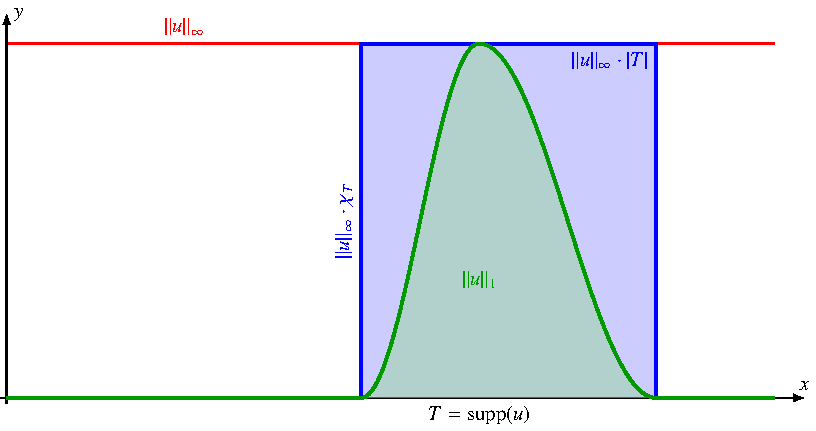
\includegraphics{chapters/060-diskret/images/traeger.pdf}
\caption{Der Träger $\operatorname{supp}u$ einer Funktion $u$ kann
als Lokalisierungsmass verwendet werden.
Jede Funktion $u$ (grün) mit Träger $T$ kann durch $\|u\|_\infty\cdot\chi_T$
abgeschätzt werden (blaue Funktion), so dass $\|u\|_1\le \|u\|_\infty\cdot|T|$
gilt.
Zwischen dem allgemeinen Lokalisierungsmass $H(u)=\|u\|_1/\|u\|_\infty$
und der Grösse des Trägers besteht also ein direkter Zusammenhang.
\label{buch:diskret:unschaerfe:fig:traeger}}
\end{figure}
